\section{Séance 4 : Internal Model Control}
\subsection{Introduction}
L'objectif de ce laboratoire est de découvrir une structure de réglage appelée structure de réglage par modèle interne ou "IMC" pour \textbf{I}nternal \textbf{M}odel \textbf{C}ontroller.\\

Le principe de cette structure de réglage est de considérer une transmisttance inverse à celle du système en amont de celui-ci. De cette façon, la transmittance totale du système est égale 1. Ainsi, un échelon en entrée se retrouvera de manière identique en sortie.\\

\subsection{Internal Model Controller}
\subsubsection{Schéma simplifié}
\begin{figure}[H]
\centering
    
\tikzstyle{block} = [draw, fill=blue!20, rectangle, minimum height=3em, minimum width=6em]
\tikzstyle{sum} = [draw, fill=blue!20, circle, node distance=1cm]
\tikzstyle{input} = [coordinate]
\tikzstyle{output} = [coordinate]
\tikzstyle{tmp} = [coordinate]
\tikzstyle{pinstyle} = [pin edge={to-,thin,black}]

\begin{tikzpicture}[auto, node distance=2cm,>=latex']
% Blocks
       
\node [input, name=input] {};
\node [block, right of=input, node distance=4cm] (system-1) {$H^{-1}(s)$};
\node [block, right of=system-1, node distance=4cm] (system1) {$H(s)$};
\node [output, right of=system1, node distance=4cm] (output) {};
		
% Basic horizontal Flow
\draw [->] (input) -- node {$y_{sp}(s)$}(system-1); 
\draw [->] (system-1) -- node {$U(s)$} (system1);
\draw [->] (system1) -- node {$y_{pv}$}(output);
     


\end{tikzpicture}
\caption{Schéma simple de la structure de réglage \textbf{IMC}}
\end{figure}

Nous retrouvons sur le schéma selon le modèle de \textit{Vander Grinten}
\begin{itemize}
\item La fonction de transfert modélisant le système 
\begin{equation}
H(s) = \frac{k \cdot e^{-sT_{m}}}{(sT_{1} + 1)(sT_{2} + 1)} 
\end{equation}

\item La fonction de transfert inverse
\begin{equation}
H^{-1}(s) = (sT_{1} + 1) \cdot (sT_{2} + 1) \cdot \frac{1}{k}\cdot e^{sT_{m}}
\end{equation} 
\end{itemize}

Cette structure implique plusieurs choses :
\begin{itemize}
\item Inversion du temps mort\\
Sauf qu'on ne peut pas inverser le temps mort (le système devrait non-causal)

\item Utilisation d'un modèle\\
Nous utilisons un modèle pour représenter le système. Cela suppose qu'il ne correspond pas exactement au comportement réel du système. Si le système est piloté avec les paramètres du modèle, il en résultera des erreurs dues aux différences entre le modèle et le système réel. Ces erreurs s'additionneront avec les autres perturbations appliquées au système. 
 
\item Degré de la fonction de transfert\\
De plus, on a un degré plus élevé au numérateur (ce qui impliquerait des impulsions de Dirac infinies en sortie) nous allons donc devoir mettre un dénominateur supérieur en filtrage pour équilibrer la fonction.
\end{itemize}

\subsubsection{Schéma usuel}
\begin{figure}[H]
\centering
    
\tikzstyle{block} = [draw, fill=blue!20, rectangle, minimum height=3em, minimum width=6em]
\tikzstyle{sum} = [draw, fill=blue!20, circle, node distance=1cm]
\tikzstyle{input} = [coordinate]
\tikzstyle{output} = [coordinate]
\tikzstyle{tmp} = [coordinate]
\tikzstyle{pinstyle} = [pin edge={to-,thin,black}]

\begin{tikzpicture}[auto, node distance=2cm,>=latex']
% Blocks
       
\node [input, name=input] {};
\node [sum, right of=input] (sum) {};
\node [block, right of=sum, node distance=3cm] (system-1) {$H^{-1}(s)$};
\node [sum, right of=system-1, node distance=3cm] (point) {};
\node [sum, right of=point, node distance=0.5cm] (sum2) {};
\node [block, right of=sum2, node distance=3cm] (system1) {$H(s)$};
\node [sum, right of=system1, node distance=3cm] (sum4) {}; 
\node [sum, right of=sum4, node distance=0.5cm] (point1) {};
\node [output, right of=sum4, node distance=1.5cm] (output) {};

\node [tmp, below of=point, node distance=3cm] (link_tmp){};       
\node [block, below of=system1, node distance=3cm] (systemm) {$H_{m}(s)$};    
\node [sum, below of=sum4, node distance=3cm] (sum5) {}; 
		
\node [tmp, below of=sum5, node distance=1cm] (link_tmp1){};
\node [tmp, below of=sum, node distance=4cm] (link_tmp2){};
		
\node [tmp, above of=sum2, node distance=2cm] (d'){};
\node [tmp, above of=sum4, node distance=2cm] (d){};
		
% Basic horizontal Flow
\draw [->] (input) -- node {$y_{sp}$}(sum);
\draw [->] (sum) -- (system-1);   
\draw      (system-1) -- node {$u$} (point);
\draw [->] (point) -- (sum2);
\draw [->] (sum2) -- (system1);
\draw      (system1) -- (sum4);
\draw [->] (sum4) -- (point1);
\draw [->] (point1) -- node {$y_{pv}$}(output);
     
\draw [->] (link_tmp) -- (systemm);
\draw [->] (systemm) -- (sum5);    
        
\draw      (link_tmp1) -- (link_tmp2);
        
% Basic vertical Flow
\draw [->] (d') -- node {$d'$}(sum2);
\draw [->] (d) -- node {$d$}(sum4);
		
\draw      (point) -- (link_tmp);
\draw [->] (sum4) -- (sum5);
        
\draw      (sum5) -- node {$\widehat{d}$}(link_tmp1);
\draw [->] (link_tmp2) -- (sum);
  
\end{tikzpicture}
\caption{Schéma de la structure de réglage \textbf{IMC}}
\end{figure}

Dans cette configuration, pour régler le problème du degré du numérateur plus élevé dans la fonction de transfert inverse, on ajoute un terme $T_{f}$. On notera que l'expression du temps mort a aussi été supprimée par rapport au problème présenté dans la section précédente.\\

La fonction de transfert inverse devient alors 
\begin{equation}
H_{mf}^{-1}(s) = \frac{(sT_{1} + 1) \cdot (sT_{2} + 1)}{(sT_{f} + 1)^{2}} \cdot \frac{1}{k}
\end{equation}

\subsection{IMC avec Simulink}
En pratique nous utilisons simulink pour contrôler le système sous une vue graphique. Le diagramme présenté plus haut devient alors la figure suivante.
\begin{figure}[H]
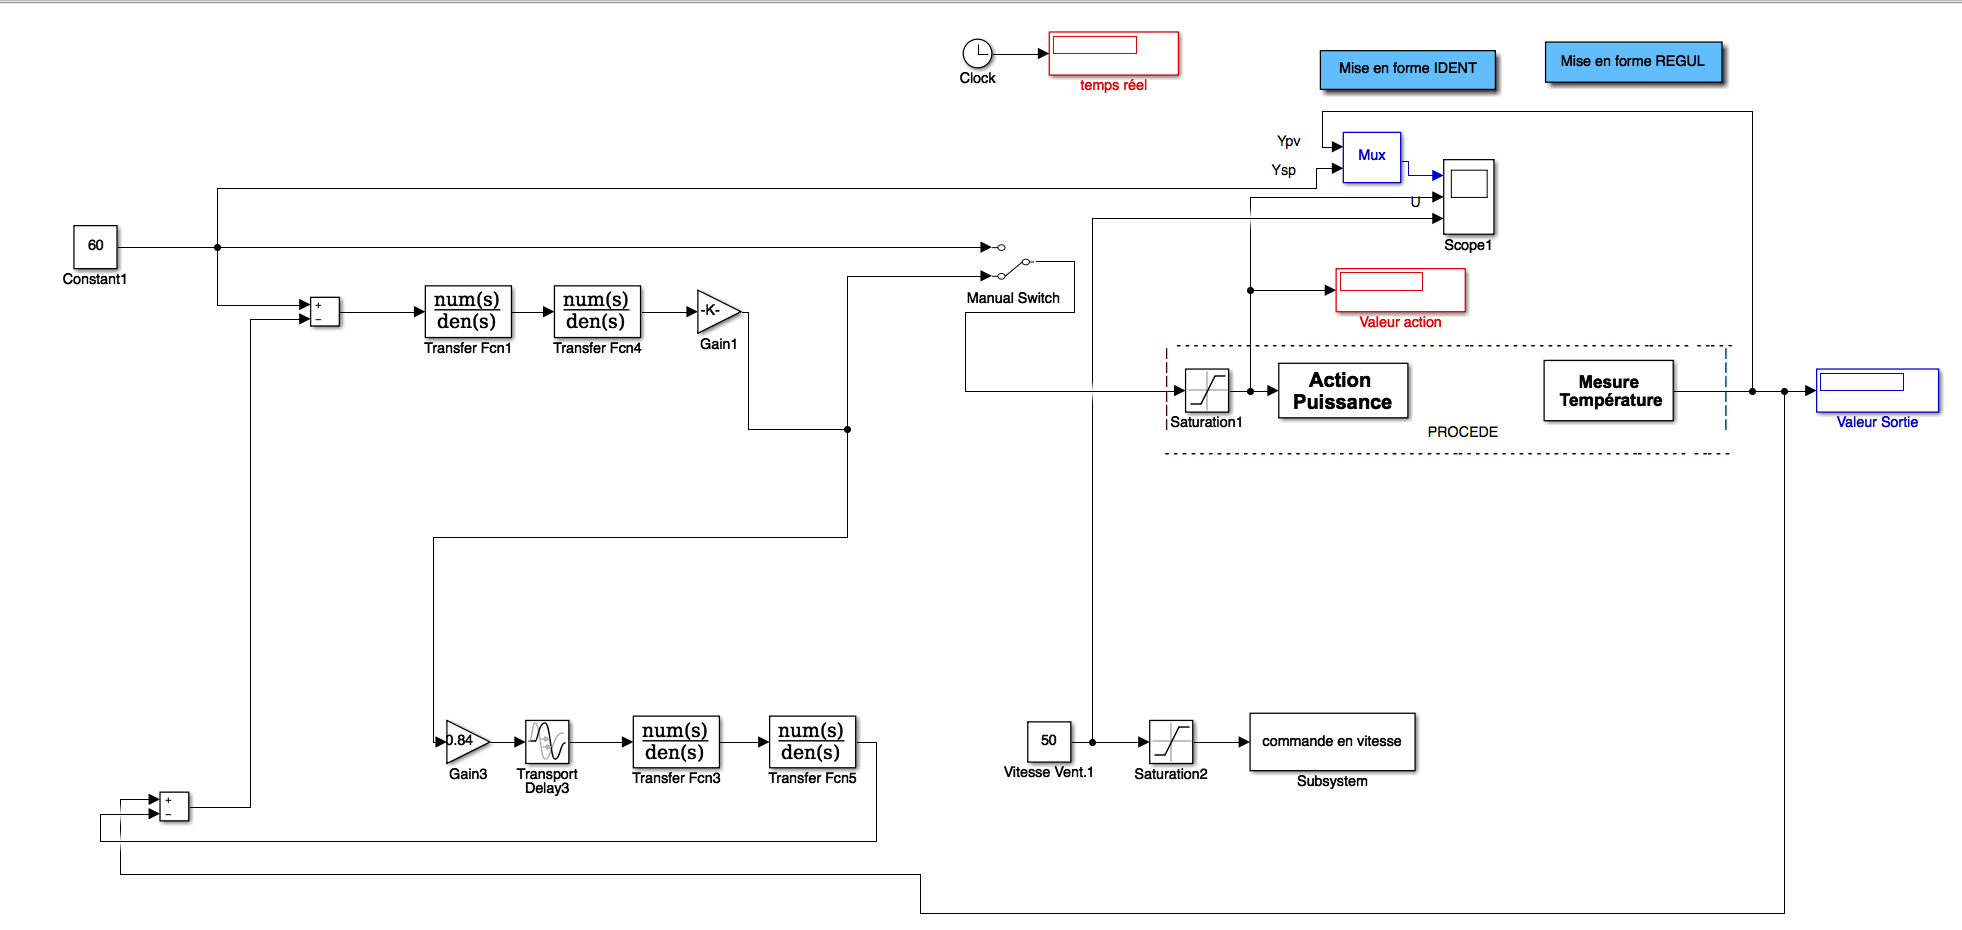
\includegraphics[width = \textwidth]{../Pictures/IMC/simulink_lab4.png}
\end{figure}
\subsection{Graphe de la réponse du système}
Lors de l'essai représenté à la figure ci-dessous, nous observons très clairement 3 périodes.
\begin{figure}[H]
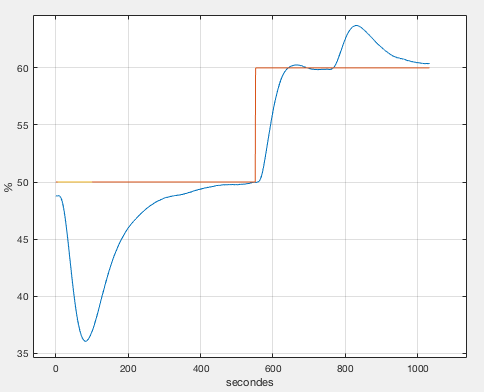
\includegraphics[width= \textwidth]{../Pictures/IMC/IMC_glob.png}
\end{figure}
Le première commence en zéro jusqu'à 580 sec et représente l'initialisation du système. Ceci correspond à la réaction du système à partir du moment où l'on applique le régulateur et nous observons que la valeur s'éloigne très fortement de la valeur de consigne avant de remonter pour venir se plaquer contre cette dernière. Cette chute rapide est due au fait que notre modèle recommence à une valeur de sortie de 0 pour monter vers la valeur de consigne demandée. En réalité, la sortie ne se trouve bien entendu pas à 0! Ceci crée un écart important entre la valeur réelle et supposée et provoque la violente chute que nous observons.

\begin{figure}[H]
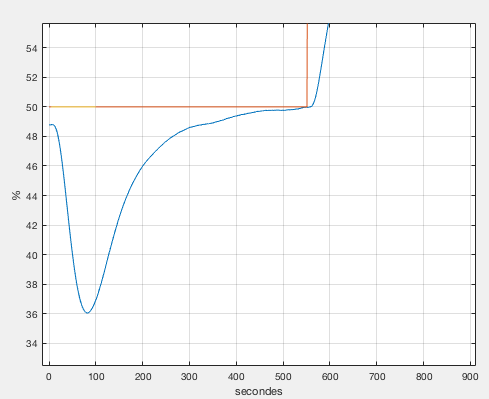
\includegraphics[width= 0.8\textwidth]{../Pictures/IMC/amorce_sys.png}
\end{figure}
La deuxième partie se déroule de 550 sec à 780 sec. Nous appliquons durant cette période un échelon de 10\% afin de vérifier la performance du régulateur en suivit de consigne. Remarquons que les performances du systèmes à ce sujet sont excellentes ! Nous remarquons en effet que le système retrouve une situation d'équilibre vers la 720ième seconde soit 140 secondes après le début de l'impulsion là où notre régulateur PID optimisé en mettait pratiquement 200 (Optimisation du régulateur - voir essai n 17 ). 
\begin{figure}[H]
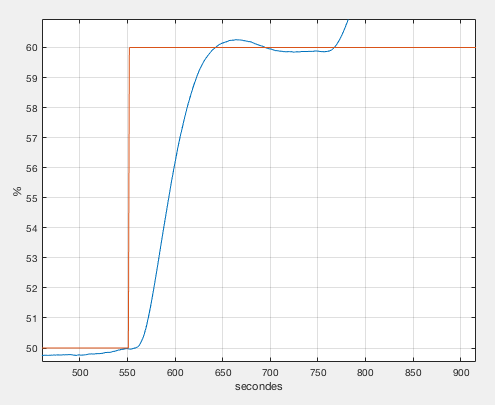
\includegraphics[width= 0.8\textwidth]{../Pictures/IMC/suivit_consigne.png}
\end{figure}
Enfin, la troisième zone va de la 760ième seconde jusqu'à la fin. Cette zone correspond à l'insertion  d'une perturbation dans le système. Dans notre cas, l'action sur l'interrupteur de la résistance chauffante a provoqué une soudaine montée en température que notre régulateur a eu beaucoup de mal à neutraliser. La valeur de la résistance ayant en effet augmenté de 4\% avant d'être atténuée contre 0,4\% pour le régulateur PID optimisé (voir figure 23- Réponse du système à une variation du ventilateur de 50\% À 60\%). Nous pouvons conclure que la réjection de perturbations est la grosse faiblesse de ce genre de régulateur. 
\begin{figure}[H]
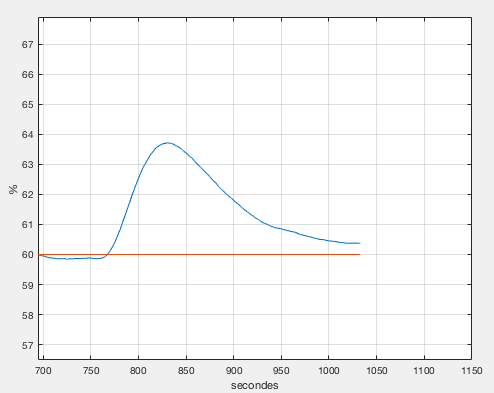
\includegraphics[width= 0.8\textwidth]{../Pictures/IMC/rej_perturb.png}
\end{figure}
Selon nous, ceci est dû au fait que en injectant une perturbation (c'est à dire en changeant la valeur de la résistance), nous recréons un système différent et au lequel notre fonction de transfert inverse n'est plus liée. Notre régulateur devient donc inadapté au système ce qui diminue très fortement ses performances. 

La situation dans laquelle nous nous trouvons est similaire à celle que nous aurions si nous n'avions rien changé au système, mais que nous avions modifier la fonction de transfert inverse "$H^{-1}(s)$". Le suivit de consigne dans ce cas-ci aurait également été beaucoup moins efficace.
\subsection{Atténuation du pic à l'initialisation du système}

Comme présenté précédement, nous constatons une importante chute de la valeur en sortie du sytème lors de l'activation du régulateur. Ceci étant dû au fait que le modèle récommence à zéro à son activation, nous pouvons aisément atténuer la chute en fixant dans le modèle une valeur proche de la valeur réelle de sortie du système lorsque que le régulateur est inactif. Cette valeur fixe nous permet de réduire l'écart entre la valeur réelle et la valeur modélisée au démarrage et donc de limiter la chute de la valeur de sortie du système. 

Bien que relativement aisée à mettre en place, nous n'avons malheureusement pas eu le temps de mettre cette technique en place lors du laboratoire du à la lenteur de notre système, ni de revenir ultérieurement en laboratoire pour refaire toute la manipulation. Nous supposons cependant à la vue des résultats des autres groupes que nous aurions atteint des résulats similaires permettant de n'avoir une chute que de quelques pourcents( voir moins) au lieux des 23 \% que nous obtenions précédement. 






